\documentclass{article}
\usepackage[utf8]{inputenc}
\usepackage{multicol}
\usepackage{lmodern}
\usepackage[T1]{fontenc}
\usepackage{mathtools}
\usepackage{amsmath}
\usepackage{amssymb}
\usepackage{graphicx}
\usepackage{mathrsfs}
\usepackage{array}
\usepackage{bm} %Bold symbols in equations
\usepackage{siunitx} %Per a poder colocar unitats en sistema internacional, com és el cas dels angstroms.
\usepackage{geometry}
 \geometry{
 a4paper,
 total={170mm,257mm},
 left=20mm,
 top=20mm,
 }
 \usepackage{esvect} %Per poder colocar els vectors
 %\usepackage[latin1]{inputenc} %fa aparèixer els caràcters


\title{\textbf{PRACTICAL SESSION 1}}
\author{\textbf{By Sergi Pradas Rodriguez} \\
\textbf{SIMCON, Engineering Physics.}}
\date{}

\begin{document}

\maketitle

\section{Fortran code to add an integer to a real number}
In this first section we present a Fortran code that adds an integer to a real number and outputs the result to an external file. The code is the following:\\
%Aqui posem la imatge del codi.
\section{Computation of Leibniz's formula}
In this section we are going to use Leibniz's formula to compute the number $\pi$. The formula is the following:
 \begin{equation}
     \frac{\pi}{4} = \sum_{k=0}^{\infty}\frac{(-1)^k}{2k+1}
 \end{equation}
And the code used is the following:\\
%Aqui posem el codi utilitzat
As it can be seen, we set a maximum tolerance for the result, so that the loop keeps going until the error with respect to the exact value of $\pi$ is smaller than such tolerance. In our case, this means () iterations.
\section{Computation of the frequency spectrum $\bf{S(\omega)}$}
In this section we are interested in computing the Fourier integral of a time-dependent correlation function $C(t)=<A(0)A(t)>$. Ignoring the normalization of the result, the expression is the following:
 \begin{equation}
   S(\omega)=\int_{0}^{\infty}C(t)cos(\omega t)\,dt
 \end{equation}
In order to make this calculation, we extract the $C(t)$ data, with time steps of $0.005 ps$, from an external file named "corr.dat", and integrate the expression via Simpson's rule:
\begin{equation}
  \int_{a}^{b}f(x)\,dx \approx \frac{\Delta x}{3} \left[ f(x_0)+4f(x_1)+2f(x_2)+4f(x_3)+2f(x_4)+ \dots +4f(x_{n-1})+f(x_n) \right]
\end{equation}
Where $\{x_0,\dots,x_{n-1}\}$ are the $n+1$ points used in the integration, and $\Delta x = \frac{b-a}{n}$ is the step distance between such equiespaced points.\\
Furthermore, in order to obtain the frequency spectrum $S(\omega)$ we perform this integration for $\omega \in [0,100] \,ps^{-1}$, for () different frequencies. \\
The code used is the following:
%Posar el codi utilitzat.
The result obtained is shown below:
%Posar figura
As can be seen from the figure, this spectrum tells us that the most important frequency components are those around the peak observed at approximately $() \,ps^{-1}$.
\section{Monte Carlo integration}
In this section we are first looking to evaluate the area between the curves $y=x^{-1}$ and $y=-x^{-1}$ within the range $x \in [-1,1]$ snd $y \in [-11,11]$. The area to compute is represented in the following figure:\\
%Posar figura
Secondly, we are interested in doing this integration for different total number of points N to analyze the method's precision by making use of the known exact result: $A_{exact}=13.5916$. The N's we are going to use are $(100,10^3,,10^4,10^5,10^6,10^7)$.\\
Furthermore, in order to perform a statistical analysis of the results, for every N we will compute the area $M=100$ times, allowing us to obtain the mean value of the area ($ <A(N)>$), and the standard deviation ($ <\sigma(N)>$):
 \begin{equation}
   <A(N)>=\frac{1}{M}\sum_{i=1}^{M}A_{i}(N) \,\,\,\,\, \& \,\,\, <\sigma(N)>=\sqrt{<(A(N)-A_{exact})^{2}>}
 \end{equation}
The code used is the following:\\
%Posar codi
And the results obtained for the mean value and standard deviation of the area as a function of $N$ and for $M=100$ are:\\
\begin{figure}[h!]
\begin{minipage}[b]{0.5\linewidth}
\centering
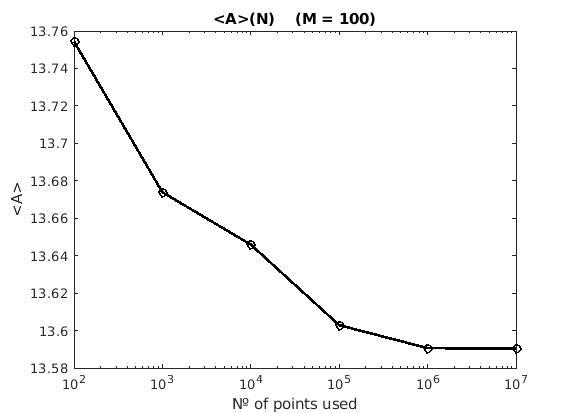
\includegraphics[width=\linewidth]{mean_A.jpg}
\label{fig:mean_A}
\end{minipage}
\hspace{0.5cm}
\begin{minipage}[b]{0.5\linewidth}
\centering
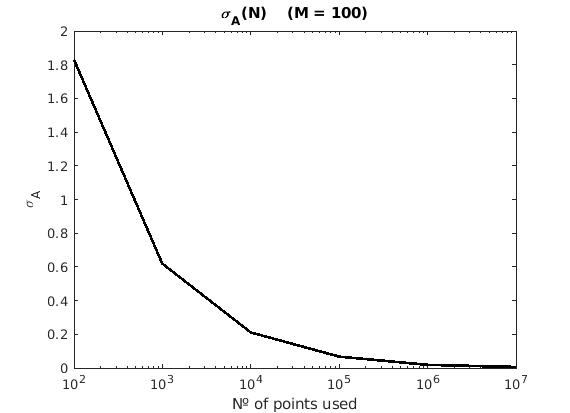
\includegraphics[width=\linewidth]{std_A.jpg}
\label{fig:std_A}
\end{minipage}
\caption{On the left, the mean value of A as a function of the number of points (N) used. And on the right, the standard deviation of such area.}
\end{figure}
\section{Integration Algorithms}
In this section we are going to analyze  three different methods of integration for resolving equations of motion: Euler, Euler predictor-corrector and Verlet. In order to do this we are going to consider an harmonic oscillator of mass $m=200 \, g$ and force constant $k=2 \,N/m$, with initial position $x_0=5 \, cm$ and $v_0=0 \, m/s$.\\
To perform this analysis we will integrate the equations of motion via Euler's method using three different time steps:$\Delta t=0.001 \,s$, $\Delta t=0.01 \,s$ and $\Delta t=0.02 \,s$; via Euler's predictor-corrector method using $\Delta t=0.02 \,s$ and via Verlet's method using $\Delta t=0.02 \,s$.\\
This way we will compare the results of the three different time steps used in the computation via Euler's method, and compare the three different methods with $\Delta t=0.02 \,s$ with the exact analytical solution. This same analysis will be performed also for the comparison of the potential (U), kinetic (K) and total (E) energies.\\
In this case we developed 4 different codes, one for each
method and one for the exact analytical solution, each one yielding a file with the information needed to plot the results. The codes used are the following:\\
%Posar els codis.
Having shown the code, the next step is to display the results. We start by showing in Figure \ref{fig:Euler_method} a comparison between the three different time steps used to solve the equation via Euler's method.\\
\begin{figure}[h!]
 \centering
  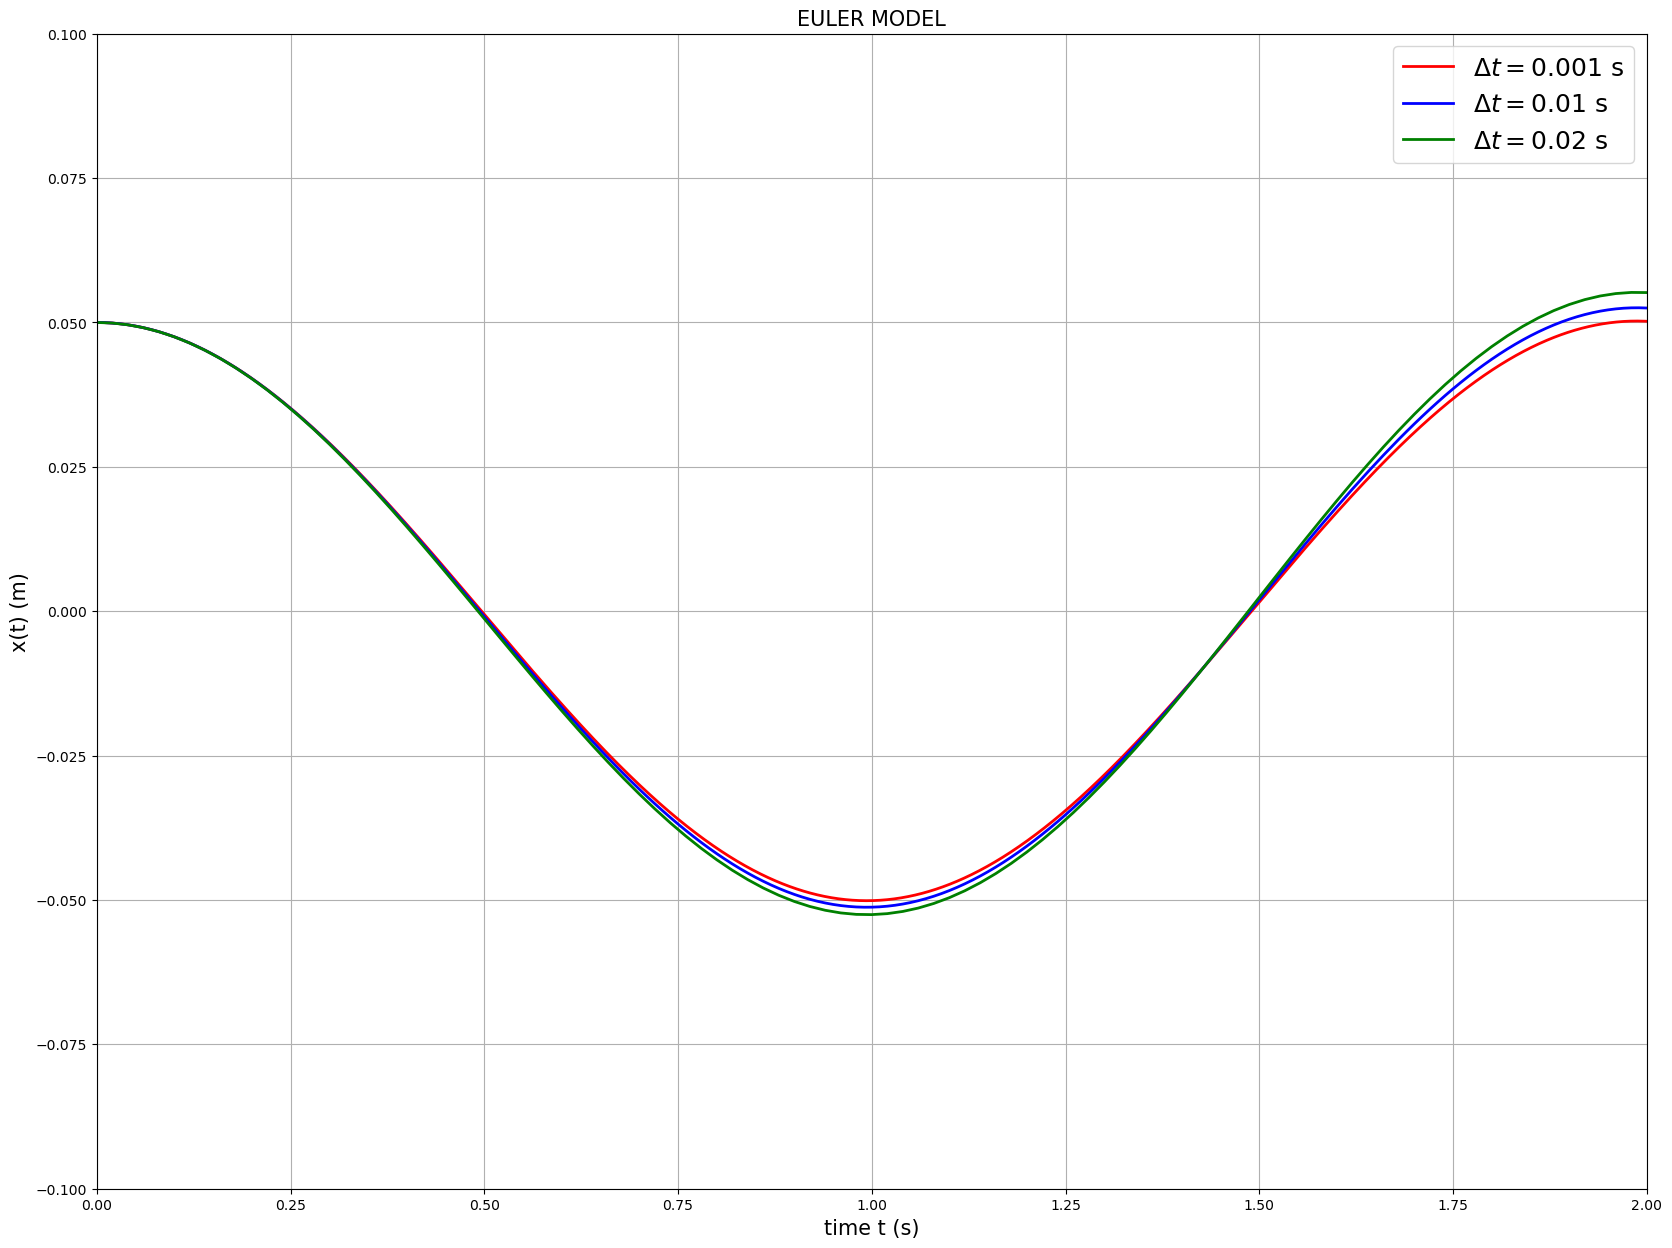
\includegraphics[width=0.7\linewidth]{Euler_eq_motion.png}
  \caption{Trajectory obtained by solving the equation of motion via Euler's method with three different time steps: $0.001 , s, 0.01 s, and 0.02 s$.}
  \label{fig:Euler_method}
\end{figure}
Next, in Figure \ref{fig:Three_methods} we show the trajectories obtained with the three different methods mentioned above when using a time step $\Delta t=0.02 \,s$ and compare them with the exact analytical solution.
\begin{figure}[h!]
 \centering
  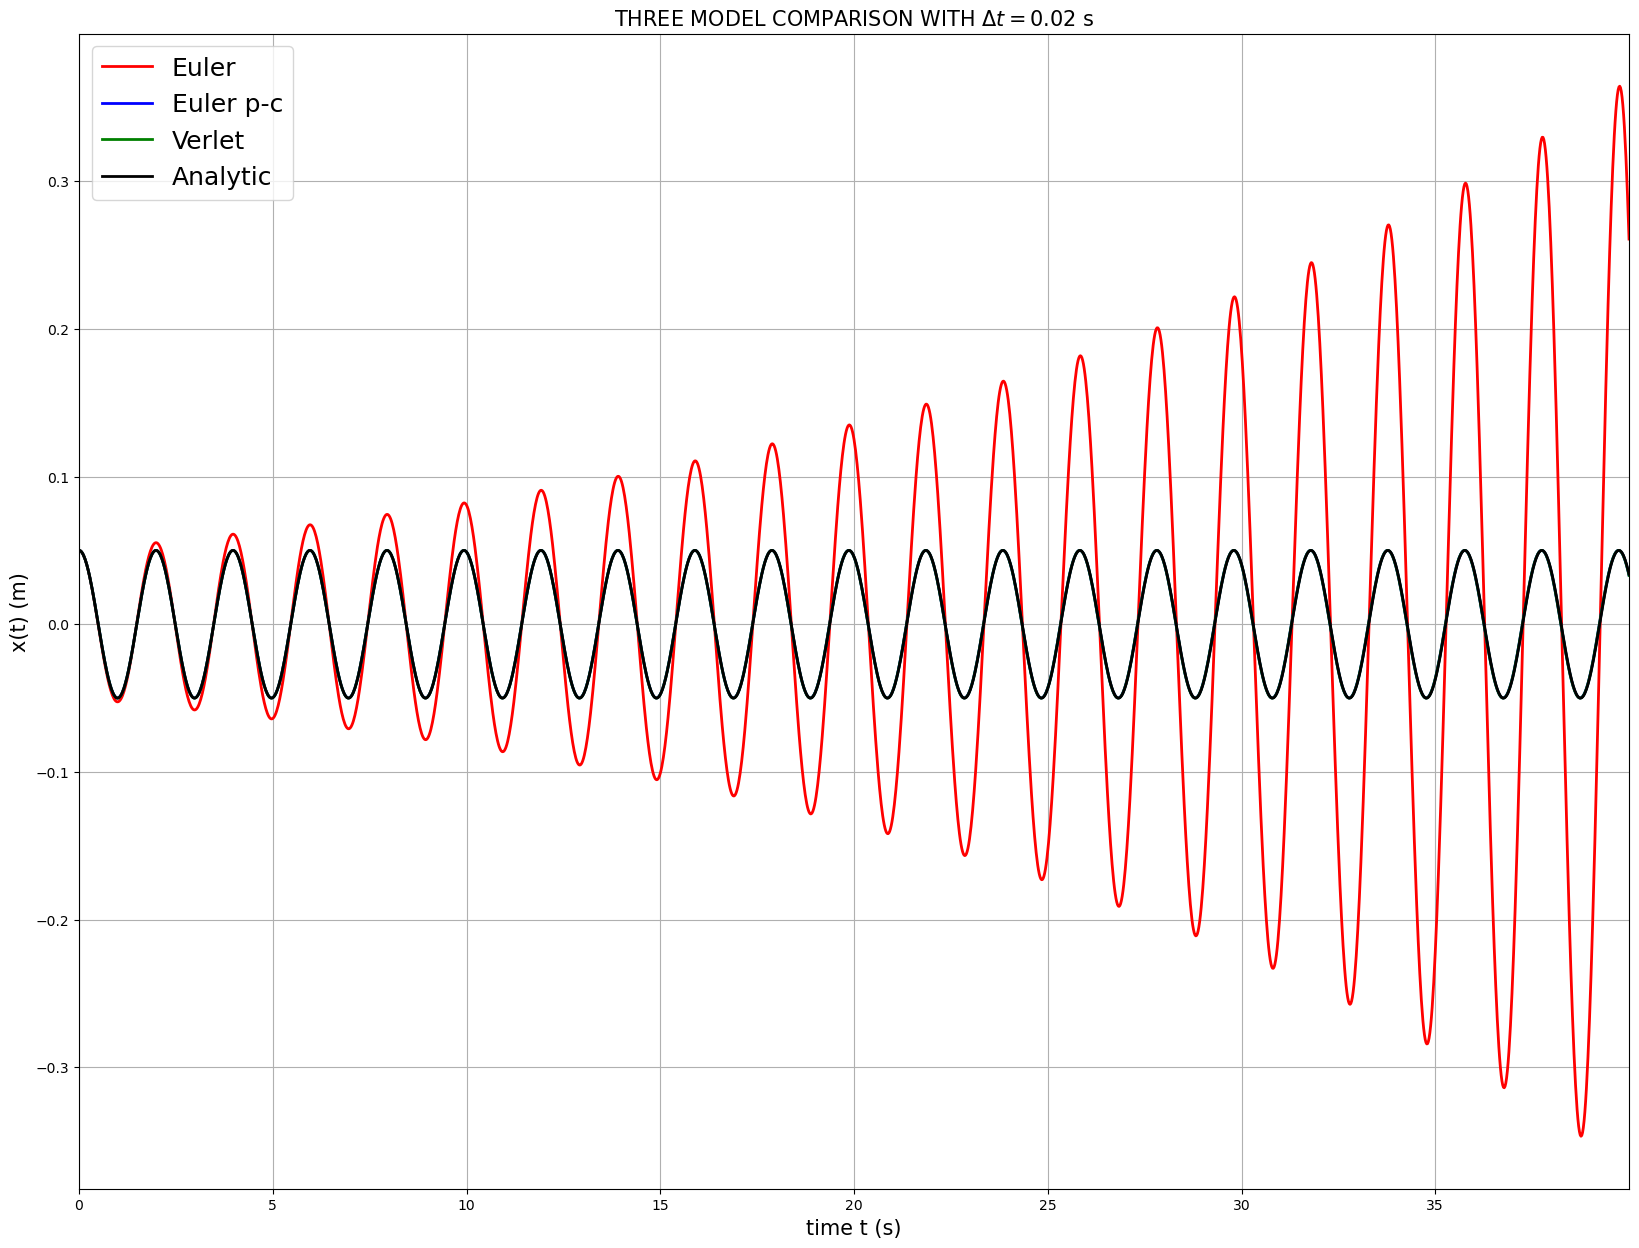
\includegraphics[width=0.7\linewidth]{Three_methods_eq_motion.png}
  \caption{Trajectory obtained by solving the equation of motion via Euler's, Euler's predictor-corrector and Verlet's method with time step $\Delta t=0.02 s$, compared to the analytical solution.}
  \label{fig:Three_methods}
\end{figure}
As it can be seen, Euler's method quickly diverges, and Euler's predictor-corrector and Verlet's method, are visually indistinguishable from the exact analytical solution. In order to show the difference more clearly, we plot, in Figure \ref{fig:Error_three_methods}, each method's error with respect to the analytical solution.\\
\begin{figure}[h!]
 \centering
  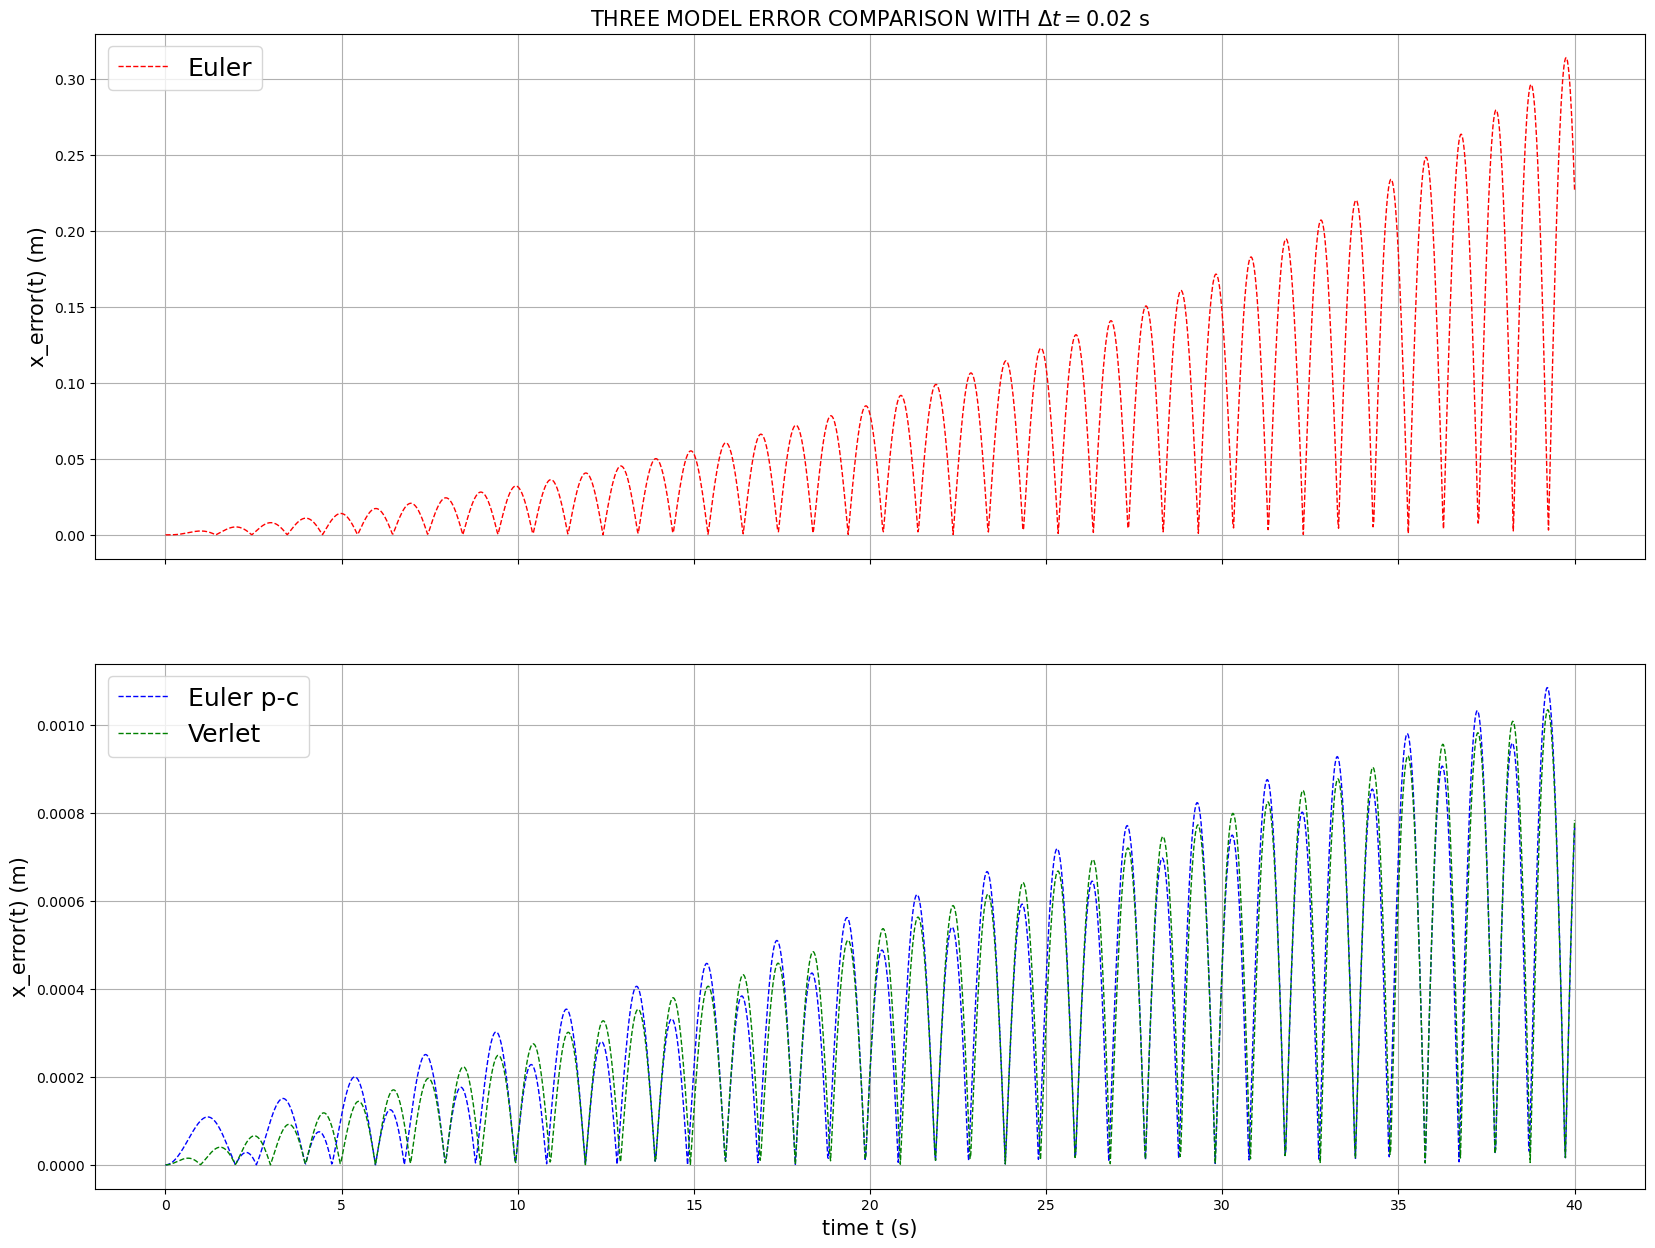
\includegraphics[width=0.7\linewidth]{Error_eq_motion.png}
  \caption{Errors obtained in the calculation of the trajectory by solving the equation of motion via Euler's, Euler's predictor-corrector and Verlet's method with time step $\Delta t=0.02 s$ compared to the analytical solution.}
  \label{fig:Error_three_methods}
\end{figure}
We can then move on to the analysis of the energies obtained for each method with $\Delta t=0.02 \,s$. We start by displaying the kinetic energy (K) and the errors with respect to the exact solution in Figures \ref{fig:K_three_methods} \& \ref{fig:K_error_three_methods}.
\begin{figure}[h!]
 \centering
  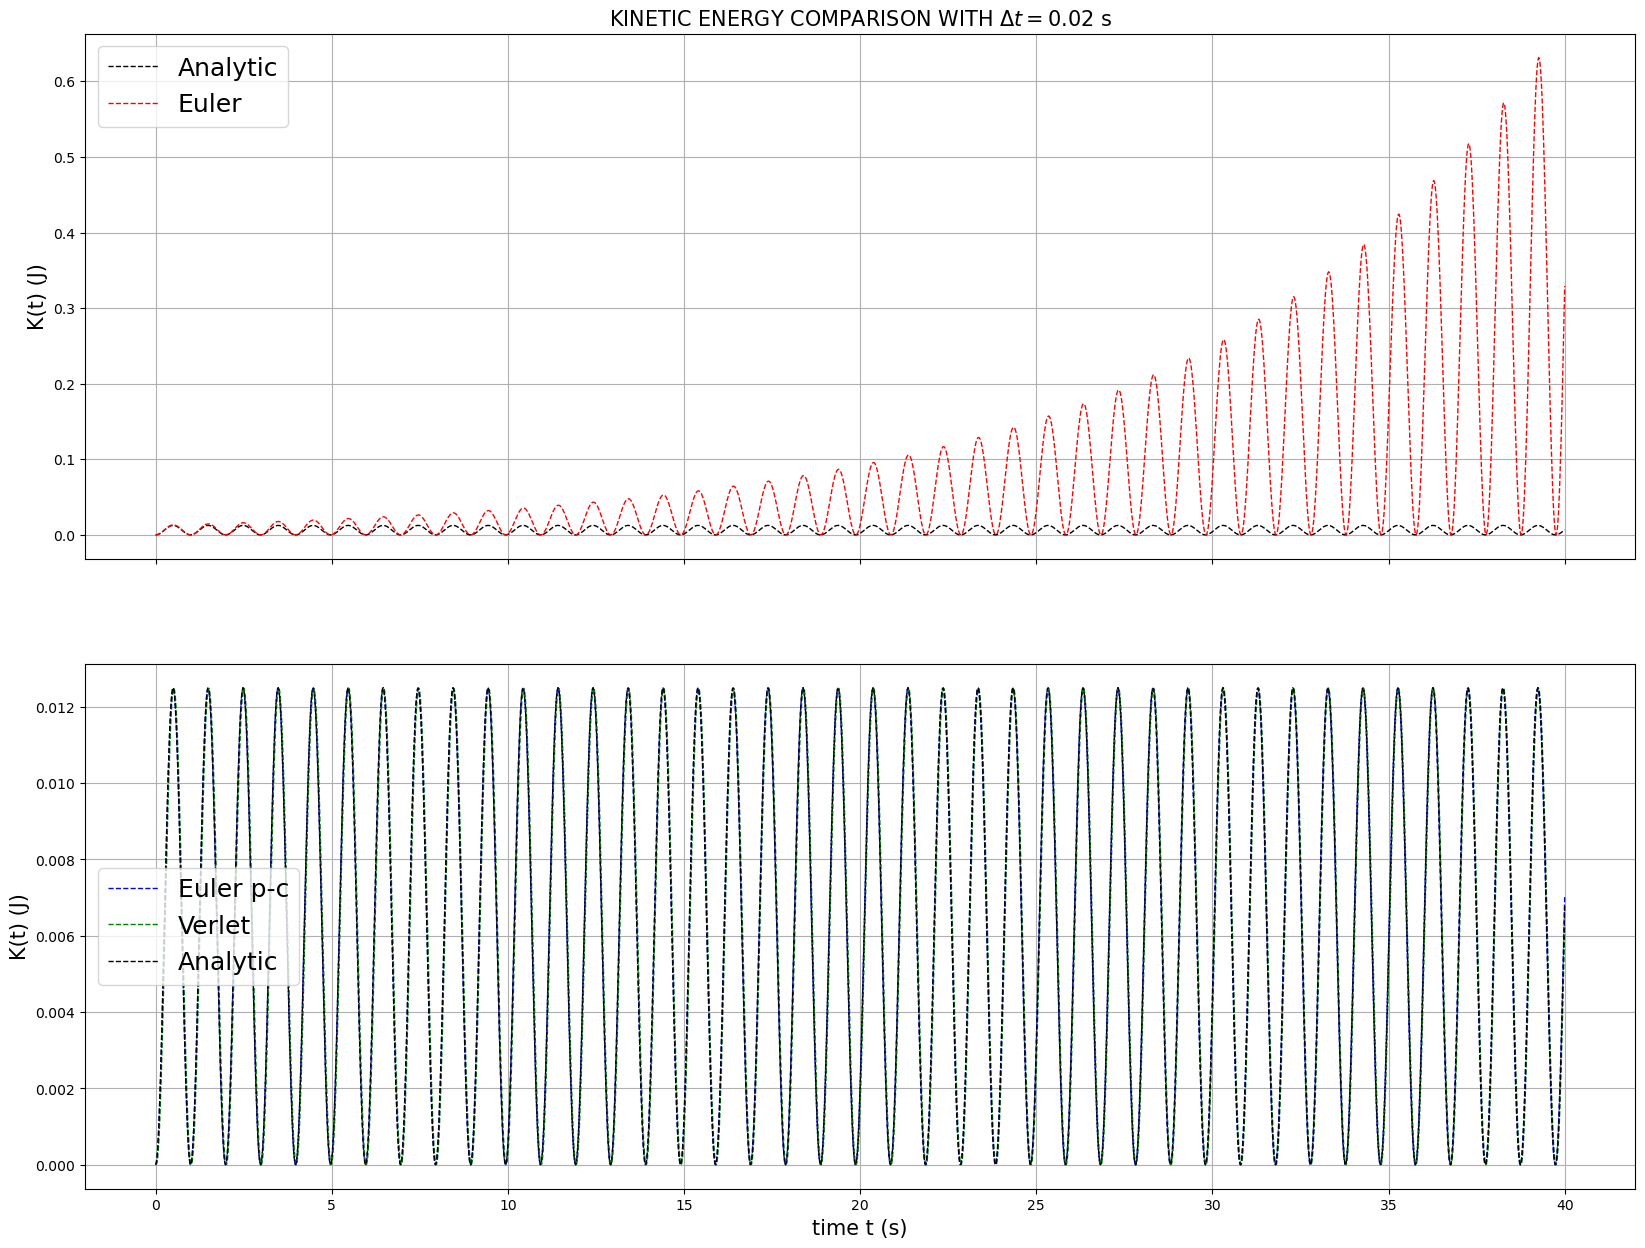
\includegraphics[width=0.7\linewidth]{K_eq_motion.png}
  \caption{Kinetic energies obtained by solving the equation of motion via Euler's, Euler's predictor-corrector and Verlet's method with time step $\Delta t=0.02 s$ compared to the analytical solution.}
  \label{fig:K_three_methods}
\end{figure}
\begin{figure}[h!]
 \centering
  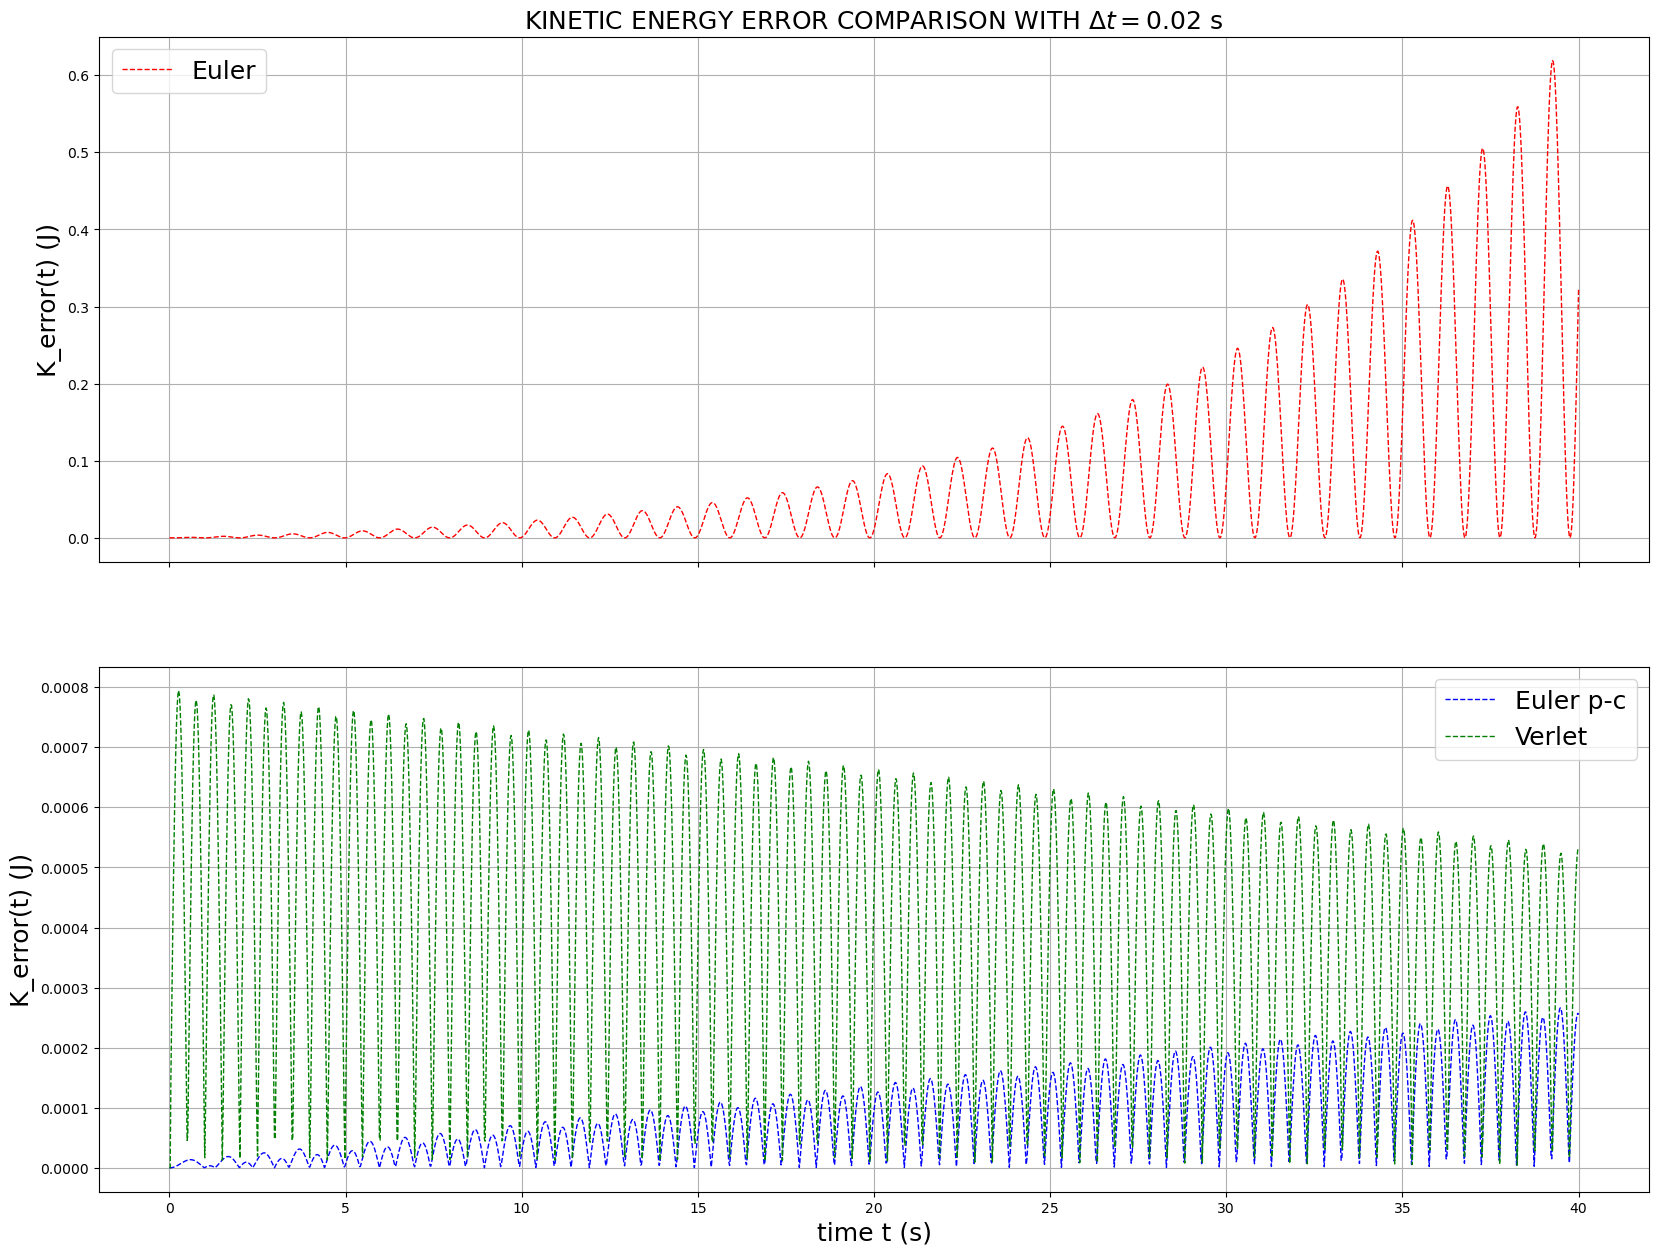
\includegraphics[width=0.7\linewidth]{K_error_eq_motion.png}
  \caption{Errors obtained in the calculation of the kinetic energy by solving the equation of motion via Euler's, Euler's predictor-corrector and Verlet's method with time step $\Delta t=0.02 s$ compared to the analytical solution.}
  \label{fig:K_error_three_methods}
\end{figure}
We follow by showing the same analysis for the potential energy (U) in Figures \ref{fig:U_three_methods} \& \ref{fig:U_error_three_methods}.
\begin{figure}[h!]
 \centering
  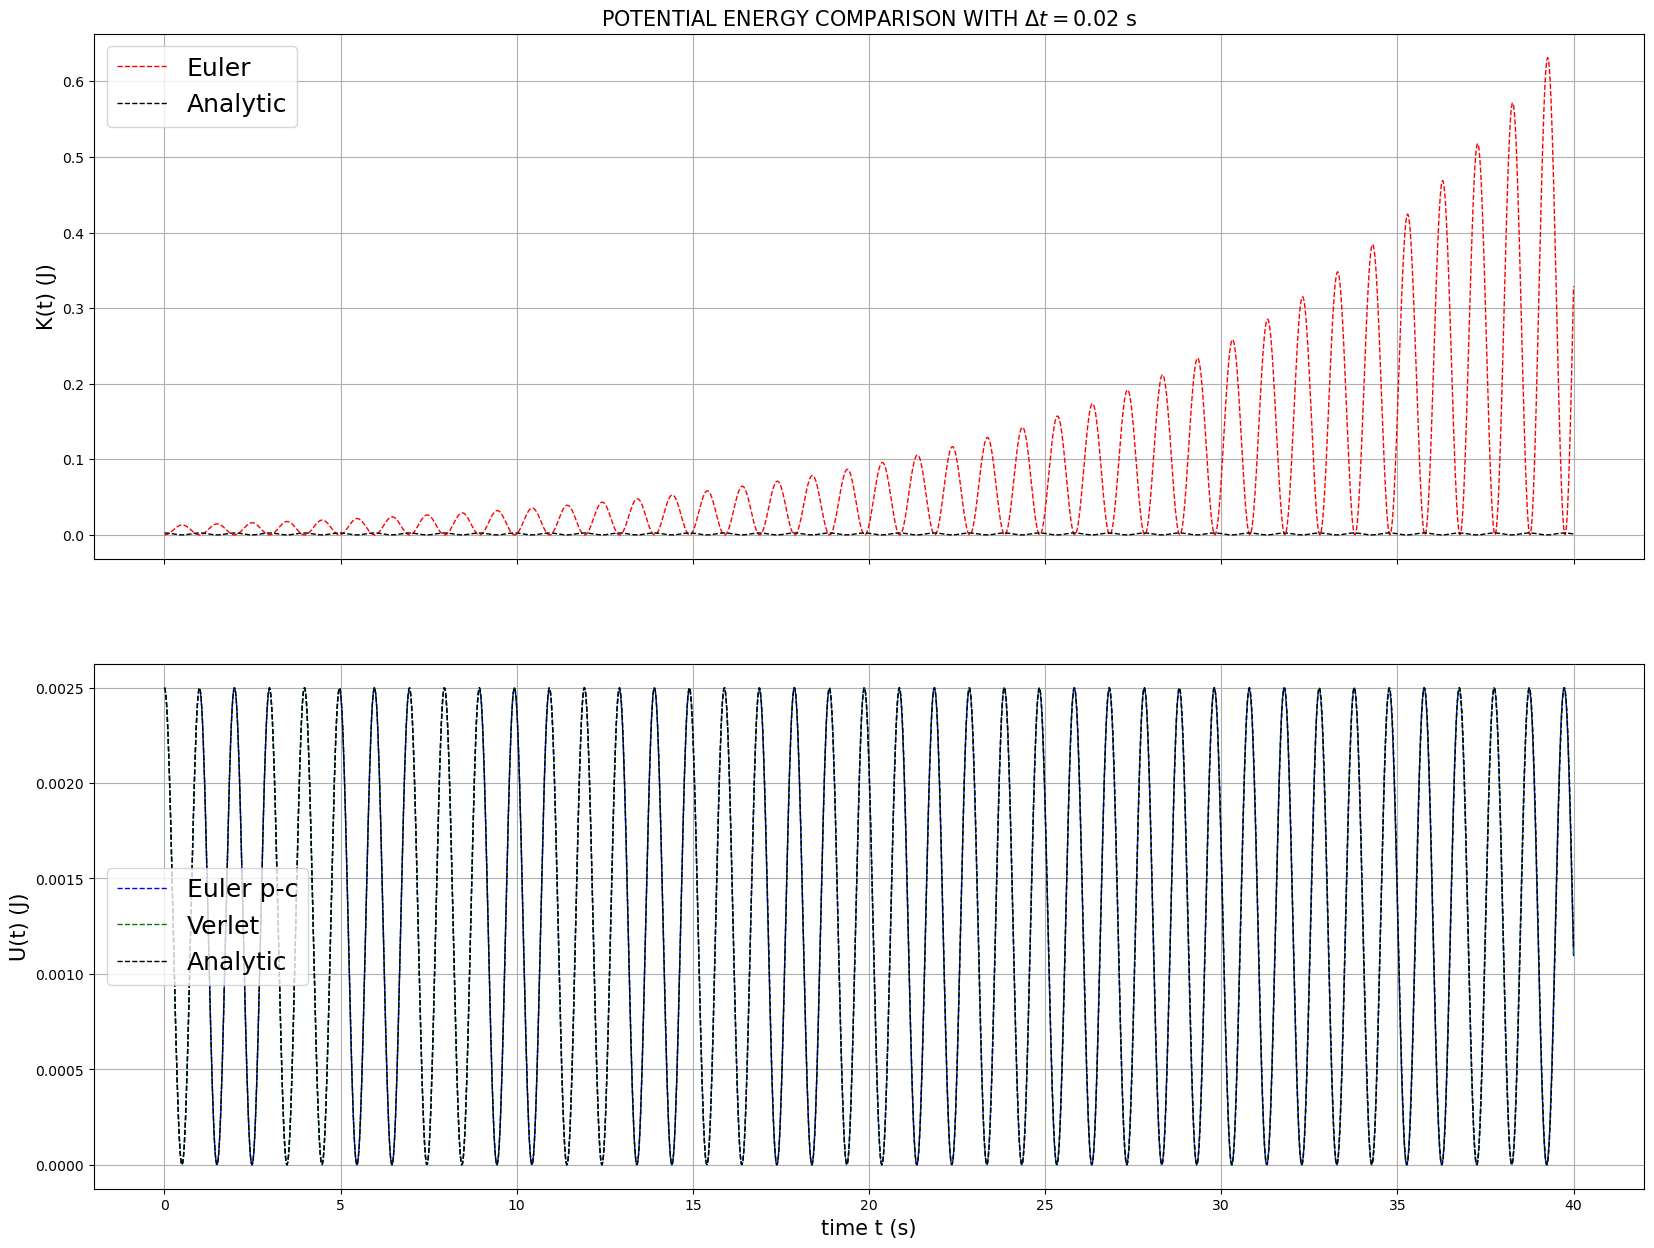
\includegraphics[width=0.7\linewidth]{U_eq_motion.png}
  \caption{Potential energies obtained by solving the equation of motion via Euler's, Euler's predictor-corrector and Verlet's method with time step $\Delta t=0.02 s$ compared to the analytical solution.}
  \label{fig:U_three_methods}
\end{figure}
\begin{figure}[h!]
 \centering
  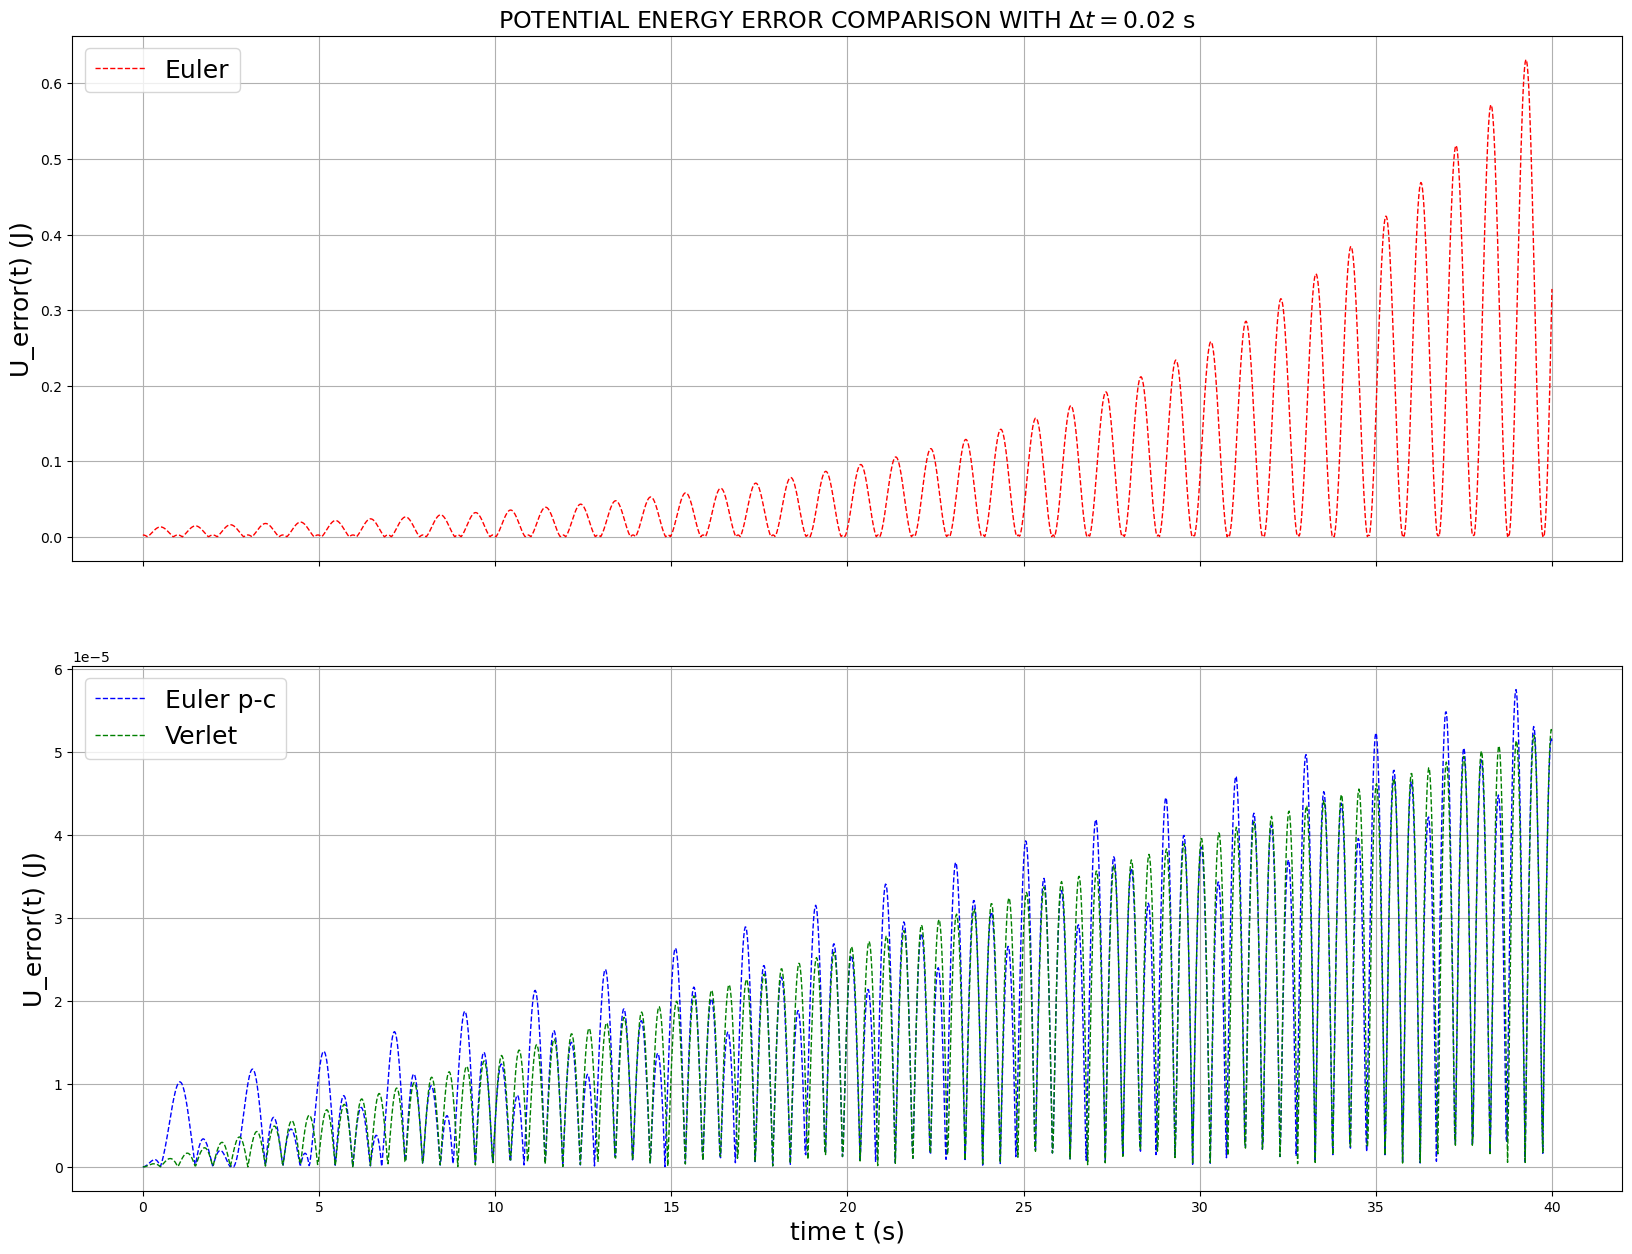
\includegraphics[width=0.7\linewidth]{U_error_eq_motion.png}
  \caption{Errors obtained in the calculation of the potential energy by solving the equation of motion via Euler's, Euler's predictor-corrector and Verlet's method with time step $\Delta t=0.02 s$ compared to the analytical solution.}
  \label{fig:U_error_three_methods}
\end{figure}
And, finally, the results for the total energy (E) are shown in Figures \ref{fig:E_three_methods} \& \ref{fig:E_error_three_methods}.\\
\begin{figure}[h!]
 \centering
  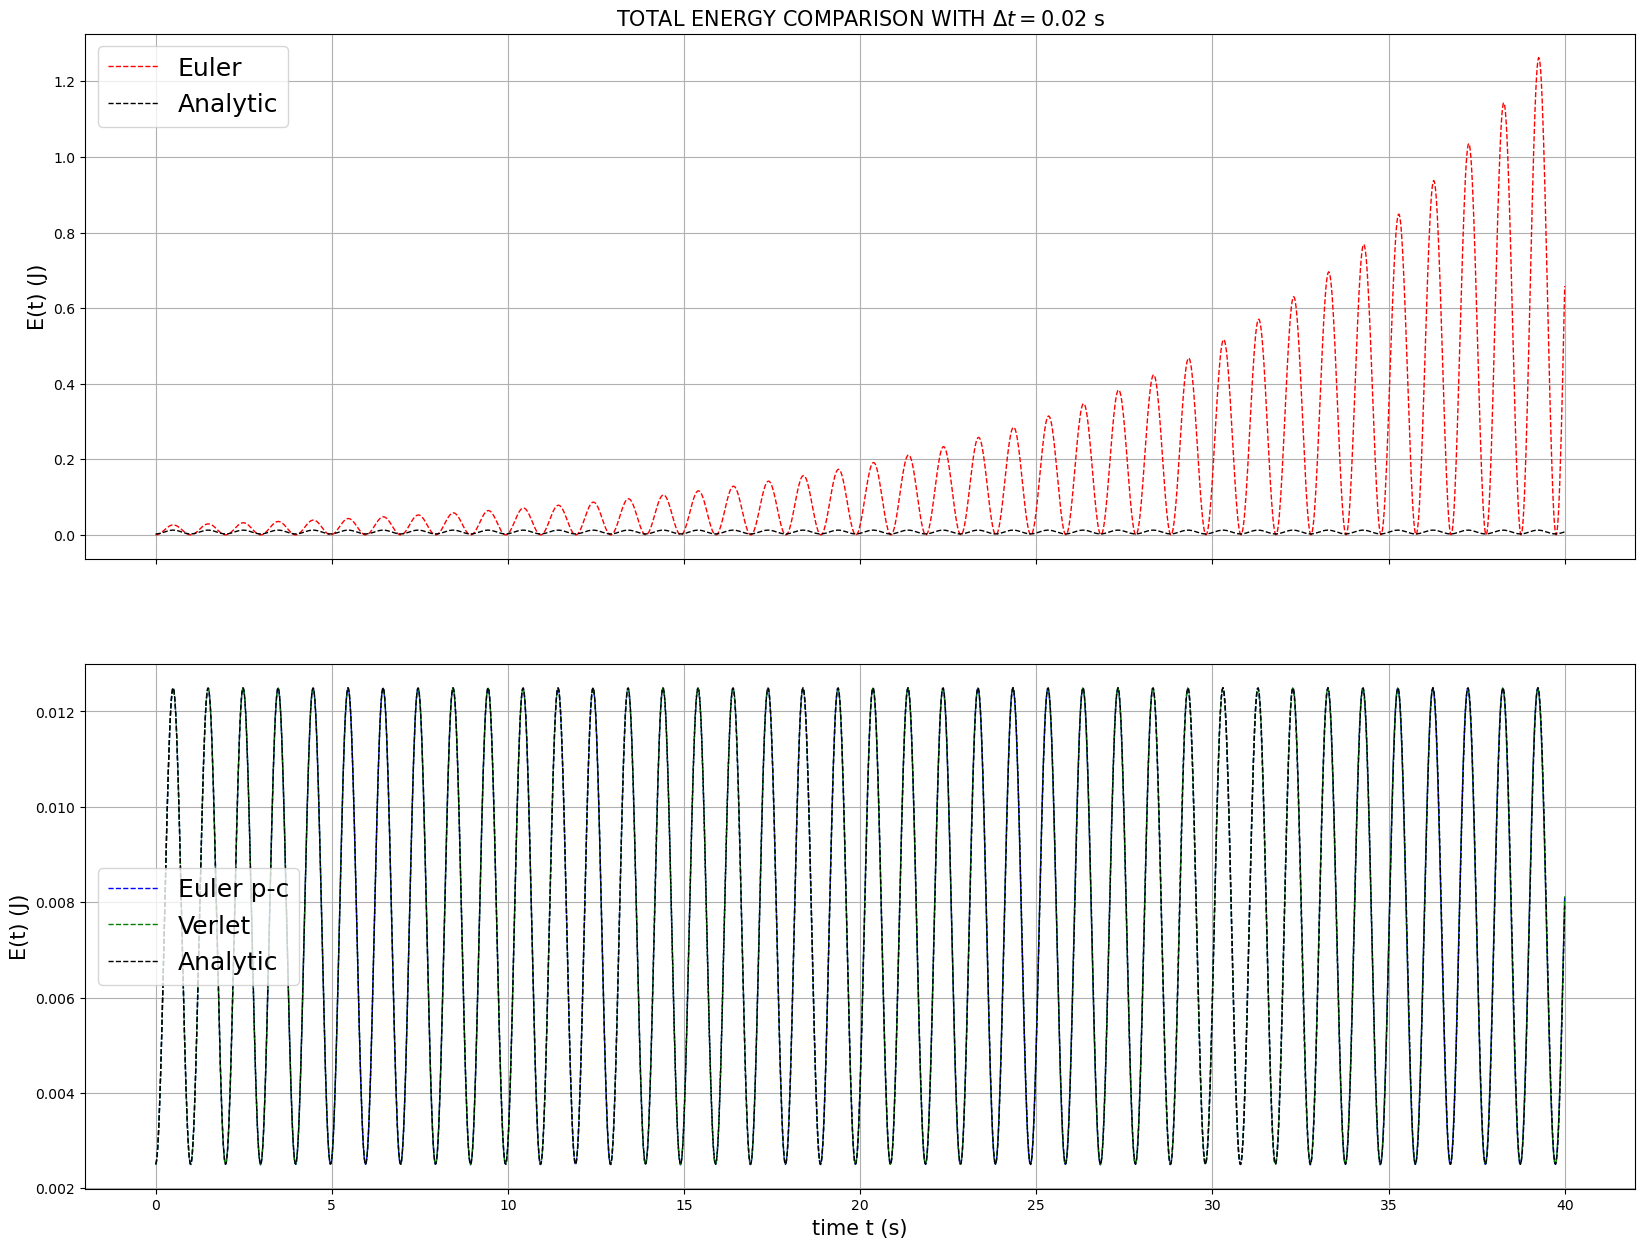
\includegraphics[width=0.7\linewidth]{E_eq_motion.png}
  \caption{Total energies obtained by solving the equation of motion via Euler's, Euler's predictor-corrector and Verlet's method with time step $\Delta t=0.02 s$ compared to the analytical solution.}
  \label{fig:E_three_methods}
\end{figure}
\begin{figure}[h!]
 \centering
  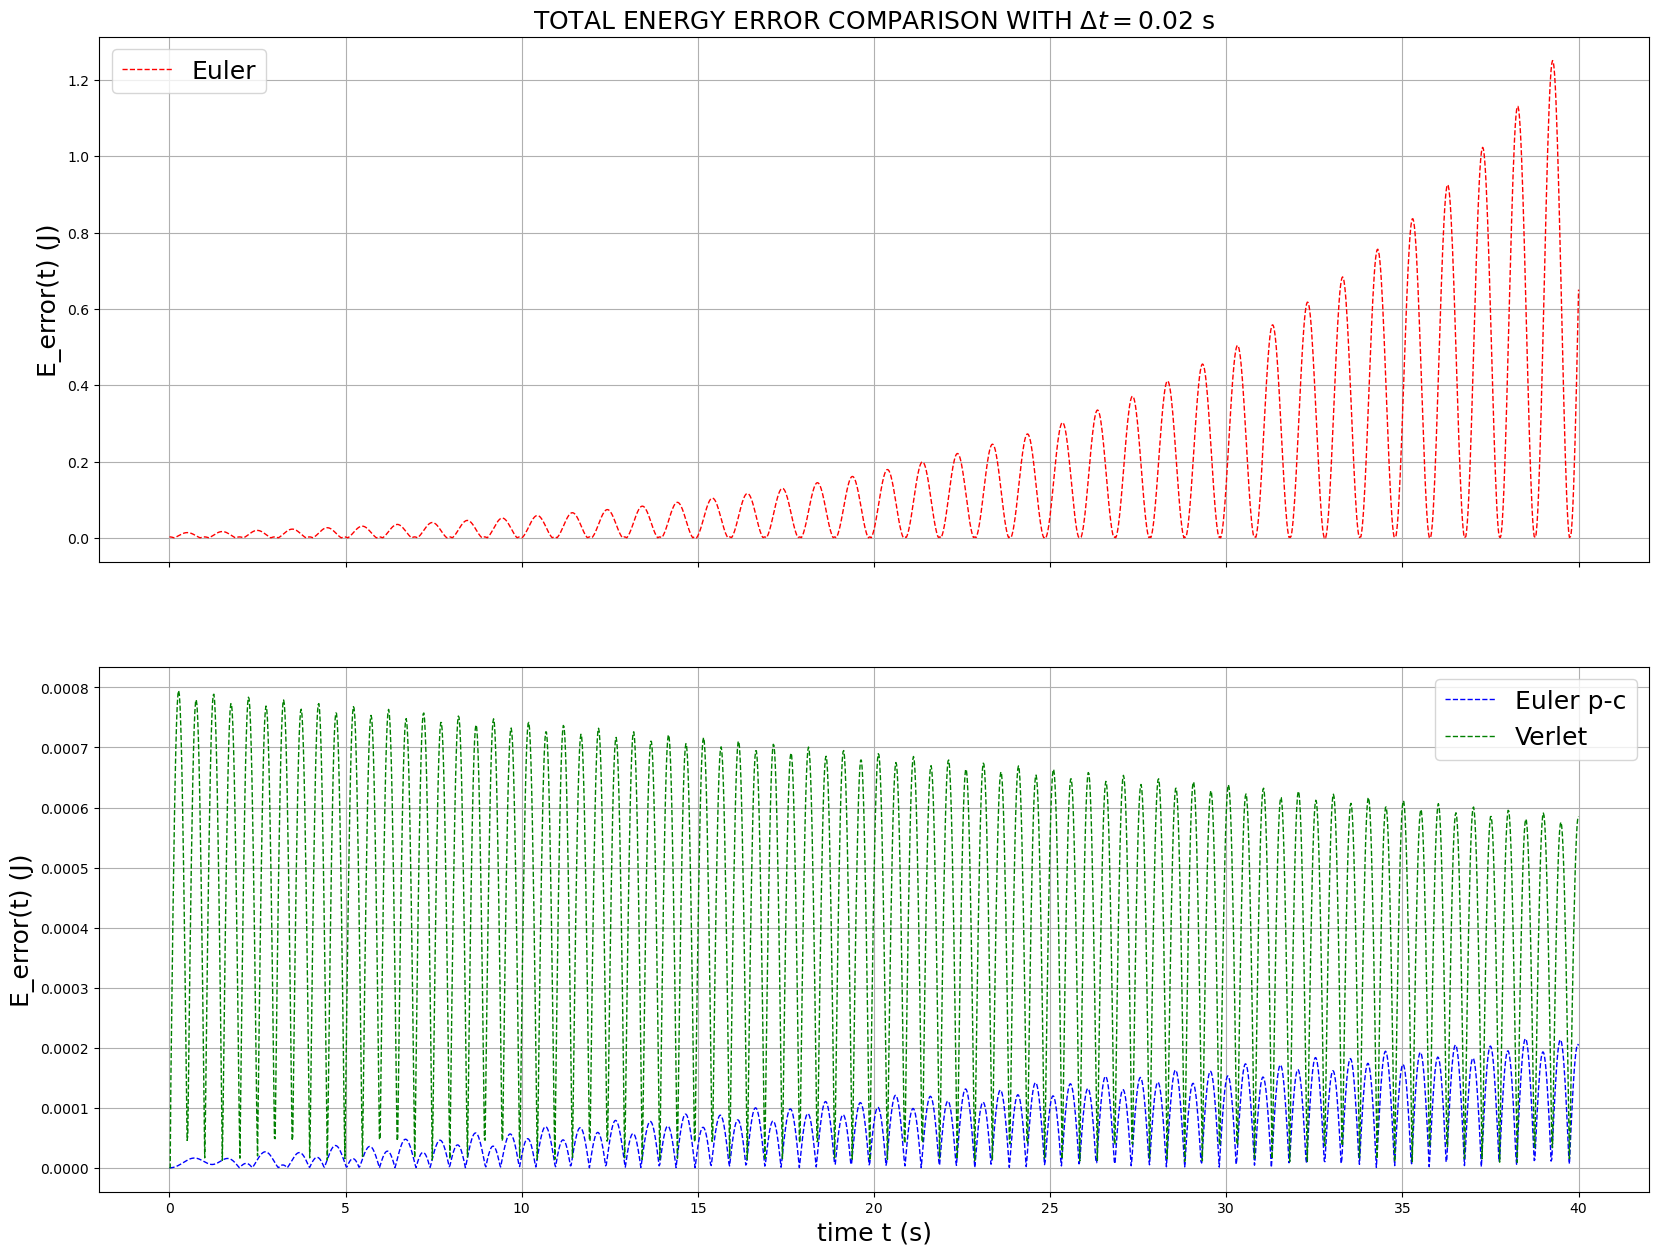
\includegraphics[width=0.7\linewidth]{E_error_eq_motion.png}
  \caption{Errors obtained in the calculation of the total energy by solving the equation of motion via Euler's, Euler's predictor-corrector and Verlet's method with time step $\Delta t=0.02 s$ compared to the analytical solution.}
  \label{fig:E_error_three_methods}
\end{figure}
From these results, we can conclude that Euler's method is by far the worst one, with Euler's predictor-corrector and Verlet's integration method yielding very similar results.


\end{document}
